% !TEX root = ../main.tex

% 附录已经设置为目录只包含章标题,章节写法与正文完全相同
\chapter{外文资料翻译}

题目:基于驾驶员—车辆—道路交互的驾驶安全场

期刊:IEEE Transactions on Intelligent Transportation Systems, 2015, 16: 2203-2214.

摘要:车辆驾驶安全受许多因素的影响,包括驾驶员、车辆和道路环境,它们之间的相互作用非常复杂。现有的评估驾驶安全性的方法仅考虑有限的因素及其相互作用,基于运动学和动力学的车辆驾驶安全辅助系统难以适应日益复杂的交通环境。在本文中,我们提出了一个新的概念——驾驶安全场。驾驶安全场利用场论来表示由驾驶员、车辆、道路状况和其他交通因素引起的风险因素。本文构建了一个统一的驾驶安全场模型,包括以下三个部分:(1)势能场,由道路上的静止物体构成,例如停止的车辆;(2)动能场,由道路上的移动物体构成,例如车辆和行人;(3)行为场,由驾驶员的个人特征构成。

\section{求和算子}

\textbf{求和算子} 是用以表达多个数求和运算的一个缩略符号,它在统计学和计量经济学分析中扮演着重要作用。如果 $\{x_i: i=1, 2, \cdots, n\}$ 表示 $n$ 个数的一个序列,那么我们就把这 $n$ 个数的和写为\equref{eq:1}:
\begin{equation}
\label{eq:1}
\sum_{i=1}^n x_i \equiv x_1 + x_2 +\cdots + x_n
\end{equation}

引用图片示例:\figref{appen:angle}

\begin{figure}[!htbp]
	\centering
	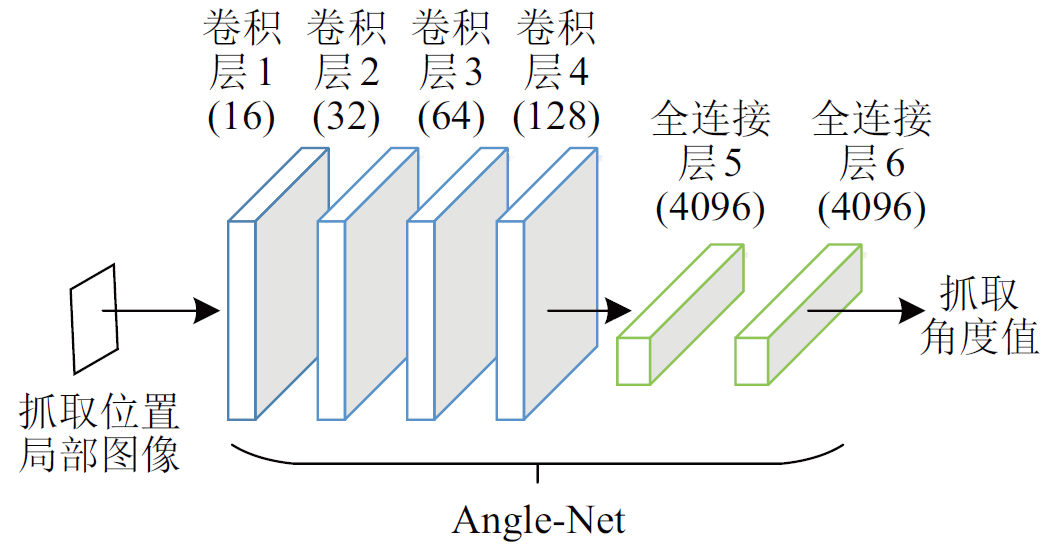
\includegraphics[width=0.6\textwidth]{3angle}
	\caption{附录插图示例:Angle-Net 结构}
     \label{appen:angle}
\end{figure}
